\documentclass[a4paper,11pt,twoside]{report}

% Gestion de la langue, des police, ligatures, etc
\usepackage[utf8x]{inputenc}
\usepackage[francais]{babel}
\usepackage[babel]{microtype}

% Marges, interlignes, graphiques et colonnes multiples
\usepackage[top=2.5cm,bottom=2.5cm,left=3.5cm,right=2.5cm,twoside]{geometry}
\usepackage{setspace}
\usepackage{multicol}
\usepackage{graphicx}


% Gestion et mise en forme de la bibliographie
\usepackage[colon]{natbib}
\usepackage{breakcites}
\usepackage{spacecites}

% Création de 2 styles d'en-têtes et pieds de page : 1 pour le corps du texte et un pour la page de garde toc, etc
\usepackage{etoolbox,lastpage,fancyhdr}

\fancypagestyle{main}{%
  \fancyhead[L]{\emph{Université de La Rochelle}}
  \fancyhead[C]{}
  \fancyhead[R]{\emph{Master SPE}}
  \fancyfoot[L]{\emph{Pierre-Louis Stenger}}
  \fancyfoot[C]{}
  \fancyfoot[R]{\thepage\ / \pageref{LastPage}}
  \renewcommand{\headrulewidth}{0.4pt}
  \renewcommand{\footrulewidth}{0.4pt}
}
\fancypagestyle{plain}{%
  \fancyhf{}%
  \fancyfoot{}%
  \renewcommand{\headrulewidth}{0pt}%
  \renewcommand{\footrulewidth}{0pt}%
}

\appto\frontmatter{\pagestyle{plain}}
\appto\mainmatter{\pagestyle{main}}

% QUelques packages utiles (couleurs, liens dynamiques dans le pdf, gestoin des unités, etc)
\usepackage[table,xcdraw]{xcolor}
\usepackage{frcursive}
\usepackage{nicefrac}
\usepackage[mediumspace,mediumqspace,Grey,squaren]{SIunits}
\usepackage[colorlinks,breaklinks,naturalnames,linkcolor=black,citecolor=black,menucolor=black,pagecolor=black,urlcolor=blue]{hyperref}


\title{{\Huge État de l'art}\\[3pc]L'apport des NGS pour inférer la structure de population}
\author{Pierre-Louis \textsc{Stenger}}
\date{}


\begin{document}
	
\onehalfspacing % interligne 1.5

%\vspace*{\stretch{1}}
%\begin{cursive}
%\textbf{In the beginning there was nothing.
%\\
%God said: 'Let there be light !'
%\\
%There was still nothing, but now you could see it.
%\\
%(Dave Thomas)}
%\end{cursive}
%\vspace*{\stretch{1}}	

% \newpage

\frontmatter

\maketitle 

\listoffigures  % table des figures
%\listoftables   % table des tableaux

\mainmatter


%\begin{BCouleur}  % Début fond gris

%\begin{abstract}
%Résumé
%\end{abstract}


%\end{BCouleur} % Fin fond gris
~~\\
\textbf{Mots clés:} \emph{NGS, Population, Génétique, Pyroséquençage, RAD-Seq, Illumina, MinION}
~~\\
%\section*{Introduction}   


\newpage

\textbf{1. Évoquer les enjeux de conservation et de protection de la biodiversité (notion d'anthropocène, 6ème crise d'extinction d'espèces, e.g. Pimm et al. 2014, Science)}
~~\\
\textbf{2. Expliquer en quoi l'inférence de la structure de populations est cruciale pour la conservation. (citer des exemples concrets)}

Estimer le taux d'échange d'individus au sein d'une population est un point central de l'écologie de l'évolution, ainsi que de ses applications en conservation des espèces et de leur management\citep{Gagnaire:2015aa}.

Regarder les flux de gènes en utilisant des marqueurs neutres permettent de voir les niveaux de différenciation entre les populations. Ces méthodes intègrent les effets des forces évolutives, sauf ceux des mutations, car leurs effets sont négligeable au regard de ceux de la migration \citep{Gagnaire:2015aa}.

La migration peut être indirectement inférée en observant la structure génétique de la population. Par exemple, les proportions génomiques des longs segments qui sont identiques entre individus provenant d'une même ou d'une différente population sont directement liés au taux de migration \citep{palamara2013inference}.  La seconde option pour détecter les événements de dispersion des individus et de trouver les distances de dispersion de la population qui peut être donné à travers l'inférence de généalogie (e.g. assignement parental) ou l'analyse de cluster (de "groupe") \citep{Gagnaire:2015aa}.

Les approches génomiques ont été suggérées comme un outil prometteur pour la pratique de la conservation pouvant améliorer la compréhension de l'inférence génétique et de fournir des nouvelles idées pour la gestion des espèces \cite{shafer2015genomics}\cite{garner2015genomics}.

Les données génétiques permettent maintenant la détection de sous-structure d'une population, de mesurer la connectivité génétique, et d'identifier les risques potentiels liés à l'évolution démographique et la consanguinité \cite{frankham1995conservation}. 

Les approches génétiques ont fait des percées qui influent sur les efforts de conservation comme par exemple, l'augmentation de la population de la panthère de Floride \textit{Felis concolor coryi} qui avaient frôlés l'extinction \cite{seal1994plan} ou encore la détection de braconnage au sein de populations menacées \cite{manel2002detecting}.

L'utilisation traditionnelle des données génétiques en biologie de la conservation a été historiquement délimité en deux domaines interdépendants \cite{frankham2002introduction}: Tout d'abord la compréhension des processus évolutifs tels que la dérive génétique, la sélection, et la migration, mais aussi la variation génétique et phénotypique des populations naturelles et de déterminer la structure de la population \cite{frankham2002introduction}; et ensuite, plus spécifiquement, décrire les effets d'une petite taille de la population sur la variation génétique et la viabilité de la population \cite{frankham2002introduction}\cite{shafer2015genomics}. 

La génomique ouvre en outre la possibilité de filtrer les individus et les populations par les "loci adaptatifs", qui est suggéré par certains comme la plus grande contribution potentielle de la génomique à la conservation \cite{mcmahon2014and}\cite{shafer2015genomics}. Par ailleurs, l'exploration de l'adaptation locale dans le monde sauvage a augmenté de manière considérable (par exemple dans des populations de corbeaux \cite{poelstra2014genomic} ou encore chez les populations de phasmes américain \textit{Timema cristinae} \cite{soria2014stick})

L'analyse ADN d'échantillons ancients (de plusieurs dizaines à plusieurs milliers d'années) peut renseigner sur des données génétiques de base dans les populations ancestrales avant des baisses démographiques actuellement \cite{bi2013unlocking}. Le moment de la fragmentation de la population et comment cela est lié à l'évolution passée de l'environnement (par exemple, l'impact anthropique ou le changement climatique) peut fournir des informations précieuses sur les processus actuels qui influent sur la viabilité de la population \cite{shafer2015genomics}.

L'inclusion de marqueurs qui reflètent l'adaptation locale augmenterait l'identification des unités de conservation et pourrait améliorer la détection de régions génomiques qui entraînerait une dépression de consanguinité \cite{allendorf2010genomics}\cite{funk2012harnessing}\cite{miller2014assessment}. Identifier des marqueurs d'adaptation seraient également utile pour la conservation des processus évolutifs (\citet{crandall2000considering} parle d'ailleurs d'ESU ("Evolutionarily Significant Units") pour classer les populations) et des gènes associés à l'amélioration de la santé de la population pourraient être propagées via une assistance humaine, y compris réaliser de l'hybridation afin de maximiser la capacité d'adaptation des populations à des environnements changeants \cite{barton2001role}\cite{nolte2010understanding}\cite{shafer2015genomics}. Cette facette de la génomique de la conservation a clairement le potentiel de fournir des informations sur les espèces,les populations, et au niveau individuel qui était inaccessible en utilisant des marqueurs génétiques traditionnels \cite{shafer2015genomics}.

Le diagnostic par les loci outliers peut être un outil précieux pour les études de suivi comme la pêche au saumon \cite{russello2012detection}, indépendamment de la signification adaptative de ces loci outliers \cite{shafer2015genomics}.

Près d'une décennie de travail sur la génomique du condor de Californie (\textit{Gymnogyps californianus}); une espèce en danger critique d'extinction; a permis de découvrir la base génétique de leur chondrodystrophie, une forme récessive et mortelle de nanisme \cite{romanov2006construction}.

Les outils génomiques peuvent aussi aider à la gestion de la pêche. Par exemple, le projet FishPopTrace s'est intéressé aux marqueurs SNP de quatre espèces de poissons commerciaux \cite{martinsohn2009fishpoptrace}: la morue \textit{Gadus morhua}, le hareng \textit{Clupea harengus}, le merlu \textit{Merluccius merluccius} et la sole \textit{Solea solea}. Ces données ont été utilisées pour décrire les populations au sein des espèces et par la suite d'identifier et de retracer l'origine géographique du poisson dans le commerce gràce aux SNP \cite{martinsohn2009fishpoptrace}\cite{shafer2015genomics}. FishPopTrace à révélé la structure de leurs populations à une échelle géographique non reconnues précédemment, ce qui conduit directement à la conservation appliquée (par exemple, l'identification du commerce illégal et les erreurs d'étiquetage) \cite{shafer2015genomics}.

~~\\
\textbf{3. Montrer en quoi c'est un challenge, particulièrement dans le domaine marin où les individus sont souvent difficile à observer, très mobiles et/ou très féconds. (citer des exemples concrets)}

L'inférence de structure des populations repose donc sur la différenciation génétique (communication personnelle; Benoit Simon-Bouhet). Cependant, l'inférence en connectivité génétique à un succés limité à cause du manque en structure génétique spatial pour les espèces à haute fécondité et à grande capacité de dispersion. Mais aussi et surtout dans les régions biogéolimités par des hotspots de différenciation génétique \citep{Gagnaire:2015aa}. 

La majorité des espèces marines combinent de nombreux traits d'histoire de vie (e.g. haute fécondité, grande taille de population, fort taux de dispersion, cycle de vie complexe...) qui produisent de mauvais patterns de différenciation génétique, avec même parfois, pas de différenciation du tout\citep{ward1994comparison}\citep{palumbi1994genetic}\citep{hedgecock2007genetic} \citep{Gagnaire:2015aa}.

De nouvelles perspectives sont offertes par l'accroissement du nombre de marqueurs dans les études de génomique des populations, et tout particulièrement celles avec un focus sur les loci influencés par la sélection \cite{Gagnaire:2015aa}.

~~\\
\textbf{4. Montrer que dans ce cadre la génétique est un outil puissant et utile. Mais montrer que dans le milieu marin, l'étude de la structure des populations se heurte à certaines limites (citer des exemples sur l'inférence de la connectivité, voir Gagnaire 2015, parler des échelles de temps/géographiques auxquelles les marqueurs classiques permettent d'accéder ou non).}

Les approches en génétique des populations offrent des méthodes d'évaluation de taux et d'échelle de dispersion (ou de migration) quand le mouvement des individus ne peut pas être mesuré par d'autres champs d'expérimentation comme la technique de CMR (Capture-Marquage-Recapture). Ces autres techniques (e.g. CMR) ne sont pas aisément applicable dans l'environnement marin, où les distributions et les voies de migrations des organismes sont cachés au yeux des humains sous la surface des océans\citep{hellberg2009gene} \citep{selkoe2011marine} \citep{Gagnaire:2015aa}.

%Les théories en génétique des populations offrent de puissant outils de travail pour estimer les distances de dispersion et les taux de migration à partir de données moléculaires\citep{Gagnaire:2015aa}.

Néanmoins, les marqueurs neutres auto-stoppeur avec des loci sous sélection peuvent donner de l'information à propos de la connectivité des patrons (patterns) dans des régions biogéographique bien mixé \citep{Gagnaire:2015aa}.

De plus, les loci outlier peuvent permettre de délimiter de manière pertinente des unités de conservations, ainsi que de mesurer des taux de connectivité entre des régions éco-géogrpahiques \citep{Gagnaire:2015aa}. 

Alors, les grandes bases de données de génomique des populations peuvent maintenant être utiliser pour étudier la connectivité des populations marines \citep{Gagnaire:2015aa}.

Il est aussi possible d'inférer la connectivité génétique en usant des méthodes indirectes. Le modèle d'IBD (Isolation By Distance) peut être utilisé pour estimer l'augmentation de différenciation génétique avec un accroissement des distances géographiques entre les populations \cite{rousset1997genetic}, ou entre les individus \citep{rousset2000genetic} quand la dispersion est spatiallement limité. Cependant, les mesures de la structure génétique ne traduisent pas facilement les taux de migration \citep{whitlock1999indirect}\citep{marko2011complex}\citep{Gagnaire:2015aa}. Un FST bas ne doit pas nécessairement signifier que la migration est forte comme la différenciation génétique est influencée par la taille efficace (Ne) et le taux de migration (m). De plus, l'estimation de la dispersion dépends d'autres paramètres comme les autres forces évolutives. Dans ce cas, les effets de la dérive génétique doivent être estimés indépendamment (généralement en estimant la densité), ce qui permet d'inférer la dispersion sous le modèle d'IBD \citep{pinsky2010using}. L'avantage de l'IBD est qu'il ne requière qu'un petit jeu de données pour tourner. Les méthodes d'inférence de population avec des méthodes indirectes échouent néanmoins sur certains points. Si la dérive génétique est trop faible pour générer une différenciation de la population, la dispersion ne peut pas être inférée en usant un modèle qui relie la balance migration/dérive \citep{Gagnaire:2015aa}. Mais, comme nous l'avons vu plus haut, ce problème est souvent rencontré avec des espèces avec des tailles de population très large, comme les poissons marins ou les invertébrés \citep{dewoody2000microsatellite}\citep{mccusker2010positive}. Par exemple, il n'y a pas de différenciation génétique détectable dans les populations californiennes de la moule \textit{Mytilus californianus} sur près de 4000km \citep{addison2008range}. En outre, des espèces avec des tailles de populations importantes peuvent montrer des pattern de structure génétique qui ne présentent pas d'équilibre mutation-migration-dérive. Les estimateurs indirects de leur dispersion sont alors basés sur différentes méthodes statistiques qui évoluent à leur propre vitesse de différenciation \citep{Gagnaire:2015aa}. 

Il est aussi possible d'inférer la connectivité génétique en utilisant des méthodes directes. Ces méthodes dont généralement plus intuitives que les approches par méthodes indirectes, il faut faire attention à bien regarder les erreurs de type I (mauvaise identification d'un individu comme étant un immigrant par exemple). Mais elles sont appliquées avec succés pour les espèces marines \citep{Gagnaire:2015aa}. Par exemple, l'assignation génétique ("genetic assignment"), basé sur des équations de fréquences alléliques est utilisé pour connaitre la dispersion des phoques gris \citep{gaggiotti2002patterns}. Ces approches requièrent une forte densité d'échantillonnage sur une large échelle géographique, et leur application en environnement marin est limité pour les populations avec des grandes tailles ou qui ont une distribution géographique mal documenté pour permettre un échantillonnage pertinent \citep{Gagnaire:2015aa}. Bien que des études récentes ont démontré que la dispersion larval avait parfois des dispersions d'échelles spatiales beaucoup plus petites de prévues \citep{almany2007local} \citep{puebla2009estimating}. Etant donné que beaucoup d'espèces marines ont typiquement de forts taux de fécondité, des distributions larges et de grandes tailles de population \citep{palumbi1994genetic}, ces méthodes sont donc peu applicables pour la majorité des espèces marines \citep{Gagnaire:2015aa}.

L'inférence de la connectivité génétique peut aussi se réaliser avec la méthode des clusters. Quand les espèces sont subdivisées en population discrètes, il faut d'abord évaluer le nombre de population avant d'évaluer le flux de gènes \citep{waples1998separating}. La méthode des clusters peut détecter les discontinuités génétiques et les limites entre les flux de gènes pour identifier les populations (ou les "stocks") et les migrants \citep{pritchard2000inference}\citep{broquet2009molecular}. Les différentes approches du clustering (\citep{pritchard2000inference},\citep{corander2003bayesian}) ont aussi leur limites, qui partent de modèles sous-jacents \citep{franccois2010spatially}. Par exemple, les modèles d'IBD peuvent conduire à du clustering \citep{aurelle2013interplay}. La puissance du clustering augmente avec la différenciation génétique au sein des population \citep{latch2006relative}. Pour cette raison, cette méthode est adapté à l'inférence de la connectivité génétique pour des espèces qui ont des capacités de dispersion faible et une taille de population locale relativement petite, par exemple \citet{ledoux2010fine} sur le corail rouge de Méditerranée et \citet{lukoschek2012sea} sur les serpents marins. Cependant ces espèces ne sont pas représentatives de la majorité des espèces marines.


~~\\
\textbf{5. Introduire une solution possible pour dépasser ces difficultés : les NGS (c'est évidemment le gros morceau de l'état de l'art). Dans cette partie, il faudra notamment :}
~~\\
	\underline{a. Expliquer de quoi il s'agit (faire un rapide point sur les principales méthodes, pourquoi pas dans un encadré séparé)}
	~~\\
	\underline{b. Évoquer la chute des coûts qui explique que ces techniques deviennent abordables pour les études à l'échelle des populations}
	
	Nous approchons du génome à 1000 dollars \cite{hayden20141}, ce qui signifie que la génération d'informations génomique est devenue de plus en plus accessible, même pour les organismes non-modèles avec de grandes tailles grande de génome \cite{ekblom2014field}\cite{shafer2015genomics}. 
	
<< moore_scriptBSB_modifié.R [, options] >>=
	     gg4
@
	   
	   
<<echo=FALSE>>=
	   setwd("/Users/pierre-louisstenger/Documents/Cours fac/Master/S3/Stage M2/R/Moore")
	   # Importation des données
	   cost <- read.table('costseq.txt',header=T, dec=",")
	   cost

	   library(ggplot2)

	   # Get costs according to Moore's law and the real cost in 2000
	   # The cost should be divided by 2 every 2 years
	   y <- cost$Couts[1]/(2^(0:6))
	   x <- seq(2000, 2012, by=2)

	   # Compute the missing values (i.e. values for years 2001, 2003, 2005, etc)
	   out <- lm(log(y)~x)
	   y <- exp(predict(out, data.frame(x=2000:2015)))
	   x <- 2000:2015

	   moore <- data.frame(y,x)
	   ggplot(data = moore, aes(x=x, y=y)) + geom_line() + geom_point()

	   all <- data.frame(Cost = c(cost$Couts,moore$y), Year = rep(2000:2015, 2), Source = rep(c("Observé","Loi de Moore"), each=16))
	   all
	   
	   gg4 <- ggplot(data = all, aes(x=Year, y=Cost, colour=Source)) + geom_line() + scale_y_log10()
	   gg4 <- gg4 + xlab("Années") + ylab("Coût") + ggtitle("Évolution des coûts des séquenceurs entre 2000 et 2015 comparée à la loi de Moore")
	   gg4
	   
@
	   
<<echo=FALSE,cache=FALSE>>=
	  gg4	  
@


	~~\\
	\underline{c. Expliquer l'intérêt de disposer de 10aines de milliers de marqueurs répartis dans tout le génome plutôt que seulement quelques 10aines. Quels sont les verrous que cela permet de lever. Donner des exemples. C'est la partie la plus importante de cette synthèse.}
	
Plus il y a de marqueurs, plus la précision des mesures et la puissance des statistiques augmentent \citep{waples1998separating} \citep{Gagnaire:2015aa}.	
	
Les approches par NGS facilitent la découverte de nouveaux marqueurs qui sont influencés par la sélection \citep{allendorf2010genomics}\citep{stapley2010adaptation} \citep{Gagnaire:2015aa}. Les loci outlier peuvent révéler des patterns de différenciation génétique, à la place des marqueurs neutres qui sont parfois peu informatifs. Ainsi, nous avons vu que les signaux des loci outlier pourraient être utilisé pour délimiter des stocks adaptés localement et redefinir des unités de conservation \citep{nielsen2011genotype} \citep{funk2012harnessing} \citep{Gagnaire:2015aa}. Cette approche est tentante car la sélection peut être plus efficace que la dérive en opposition à l'effet d'homogénéisation des populations par la migration, en particulier quand les populations ont de grande taille efficace. Cependant, les loci outlier peuvent apparaitre suite à une large variété de mécanismes évolutifs en dehors de l'adaptation locale. Ces mécanismes évolutifs doivent donc être identifiés avant d'utiliser les loci outlier pour évaluer la connectivité \citep{Gagnaire:2015aa}. 	

Il faut garder à l'esprit que les hotspots de différenciation génétique peuvent se trouver auprès des barrières naturelles qui limitent la dispersion \citep{barton1979dynamics}, ou au travers de barrières exogènes ou endogènes de reproduction \citep{bierne2011coupling}. 

De plus, les effets indirects de la sélection peuvent révéler des structures génétiques cryptiques dû à de l'introgression originaire d'une zone de contact géographiquement distante \citep{gagnaire2011within}, ou alors dû aux gènes autostoppeurs qui sont générés pendant la propagation d'un balayage sélectif \citep{bierne2010distinctive} \citep{Gagnaire:2015aa}.

Utiliser des loci sous influence de la selection, et des loci auto-stoppeurs peut être une approche alternative à l'inférence de la connectivité marine. Les données avec nombreux marqueurs ont considérablement amélioré la puissance du scan génomique pour identifier les loci avec des niveaux de différenciation extrêmes \citep{stapley2010adaptation}. Les ``FST Outliers" supposent être directement ou, plus probablement, indirectement affecté par la sélection \citep{luikart2003power}\citep{storz2005invited}. De recentes études en génétique de la conservation ont proposé de délimiter localement des unités de gestion basées sur les signaux de ces loci outliers \citep{funk2012harnessing}\citep{nielsen2012gene}. Un problème commun rencontré dans les études de génomique des populations est que les différentes méthodes pour identifier les FST outliers détectent seulement partiellement les lots de chevauchement des loci. La méthode de detection des FST la plus commune a un fort taux de détection faux-positif sous des scenari non équilibrés \citep{lotterhos2014evaluation}, dans des populations hiérarchisés \citep{excoffier2009detecting}, et dans les patterns d'IBD \cite{fourcade2013local}. Pour contourner ces problèmes, combiner les méthodes basées sur la différenciation avec l'association du génotype et de l'environnement est suggéré comme plus fiable que l'approche des outliers \citep{villemereuil2014genome}. En outre, la sélection peut aussi avoir un effet dominant sur la diversité génétique des espèces marines, tel est le cas de populations d'épinoches \textit{Gasterosteus aculeatus} \citep{roesti2012genome} ou de encore de bar \textit{Dicentrarchus labrax} \cite{tine2014european}. 

Les clines génétiques peuvent aussi estimer les distances de dispersion. Les études sur les scans génomiques dans le milieu marin ont reporté des exemples de patterns en forme de clines sur les loci outliers, qui pourraient coincider dans l'espace avec un changement de gradient environnemental, d'écotones, de barrières biogéographiques... (\citep{murray2006genomic}\citep{colbeck2011historical}\citep{gagnaire2011within}\citep{limborg2012environmental}) Les formes de clines peuvent être déterminés basiquement par la balance entre la migration et la sélection. Les études de génomique des populations ont maintenant le pouvoir de détecter des loci montrant des variations clinales dans des espèces que l'on croyaient être génétiquement homogènes. La probabilité de découvrir de nouveaux cas d'adaptation locale avec les clines, et des zones hybrides cryptiques est donc grande \citep{bierne2011coupling}. 

La fréquence des allèles varient selon une courbe sigmoïde de la distance géographique, sans nécessairement trouver une fixation d'un allèle si la sélection ne peut pas purger l'afflux de génotypes maladaptés. Les clines d'adaptation local peuvent être utilisés pour estimer la distance de dispersion, si le coefficient de sélection peut être mesuré, ce qui représente actuellement un challenge. La mesure de la sélection peut parfois être obtenue en utilisant des populations expérimentales ou en comparant la fréquence du génotype entre les larves et les adultes collectés d'une même cohorte. Ces clines d'adaptation locale peuvent offrir des alternatives pour estimer la migration des espèces marines avec un grand flux de gènes, en gardant à l'esprit que les modèles sous-jacents supposent que chaque cline évolue indépendamment. Par exemple, un scan génomique de grande densité réalisé chez \textit{Drosophila melanogaster} a révélé la présence de clines latitudinaux \citep{fabian2012genome} qui se chevauchent géographiquement, avec des clines qui ont été attribués à de l'adaptation locale \citep{berry1993molecular}. Comme pour la drosophile, des clines dits "classiques" ont été retrouvés dans les organismes marins, comme le cline du gène Ldh chez le poisson-killy \textit{Fundulus heteroclitus} \citep{powers1978biochemical} qui s'est finalement avéré être dû à une zone de contact secondaire \citep{durand2009spatial}. 

Les clines dû au contact de zones entre des taxa hybridés sont des zones hybrides \citep{murray2006genomic}. Dans ces clines, chaque locus cumule les effets indirects de la sélection d'un autres loci et les effets de son propre coefficient de sélection \citep{barton1983multilocus}\citep{kruuk1999comparison}. L'association parmis les allèles sous sélection dans les zones hybrides peuvent alors être utilisés pour inférer la dispersion \citep{barton1993genetic}.

Utiliser l'assignation génétique individuel ("individual genetic assignment") est une approche conceptuellement différente pour estimer la connectivité dans les zones de contact. Cette approche est très similaire à l'estimation directe de la connectivité génétique et prend l'avantage considérable de prendre en compte les différences génétiques entre des populations ou des espèces des deux côtés de la zone hybride \citep{Gagnaire:2015aa}. Cette approche est utilisé pour estimer l'origine de la dispersion de larves, comme par exemple celles de la moule bleue \textit{Mytilus edulis} \citep{gilg2003geography}. 

Estimer la connectivité d'une population est souvent nécessaire en dehors de ces régions singulières, par exemple quand il est nécessaire de déterminer s'il y a une dispersion limitée entre les populations dans les zones délimitées par des limites écologiques ou biogéographiques, ce qui est une préoccupation relativement commune pour les questions de gestion de conservation \citep{allendorf2010genomics}. Une solution potentielle, quand l'équilibre migration-dérive n'est pas informatif, est de chercher des preuves de la structure spatiale dû par une introgression \citep{gagnaire2011within}. Utiliser le ratio introgression/homogénéisation permet de montrer que les taux d'introgression sont variables entre les loci et peut donner les moyens de détecter une faible barrière au flux de gènes, même lorsque l'introgression a commencé des milliers de générations dans le passé \citep{Gagnaire:2015aa}.

Les queues d'introgressions peuvent être aussi influencés par une sélection agissant hors de la zone de tension. Dans ce cas, le gradient de la fréquence de l'allèle dans les espèces introgressés peut être accentuée par un gradient de sélection (par exemple un gradient de l'environnement). En effet, les zones de contacts secondaires coïncident généralement avec des gradients environnementaux \cite{bierne2011coupling}. De plus, les queues d'introgression peuvent être couramment rencontrées dans les régions biogéographiques séparées par des limites environnementales, comme pour la mer Baltique \citep{Gagnaire:2015aa}. Ces mécanismes montrent combien il est important d'échantillonner non seulement l'ensemble de l'aire de répartition d'une espèce, mais aussi les populations divergentes, ou alors les espèces qui sont étroitement liés et qui vivent en parapatrie ou en sympatrie, avant d'interpréter les modèles de variation génétique spatiale \citep{gagnaire2011within}\citep{cullingham2013effects}\citep{gosset2013differential}\citep{Gagnaire:2015aa}. Maintenant que les outils des NGS commencent à révéler les îlots génomiques de différenciation entre les espèces cryptiques qui étaient auparavant considérés comme des populations de la même espèce \citep{hemmer2013genomic}\citep{karlsen2013genomic}\citep{tine2014european}. Les polymorphismes situés dans la périphérie de ces îles pourraient devenir un nouveau type de marqueurs relativement puissant qui permettraient de déduire la connectivité au sein des espèces \citep{Gagnaire:2015aa}. 

Cependant la création de loci outlier peut aussi être du aux allèles autostoppeur dans une population spatiallement subdivisée. Ce processus laisse une empreinte au niveau des marqueurs neutres dans le voisinage chromosomique de l'allèle qui a été balayé. Lorsque la différenciation génomique globale est faible (ce qui est généralement le cas dans les espèces marines), ce processus génère un niveau élevé de différenciation des deux côtés du locus sélectionné \citep{bierne2010distinctive}. En effet, la recombinaison rompt progressivement l'association entre le lieu choisi et le lieu neutre auto-stoppeur, tandis que l'onde de balayage se propage \citep{Gagnaire:2015aa}. Par conséquent, l'effet de l'auto-stop est fort dans le berceau de la mutation qui est favorable, alors qu'il se ramollit progressivement à mesure que l' onde se déplace \citep{Gagnaire:2015aa}. Il n'existe que quelques exemples d'études s'ayant penché sur ce sujet, dont celui de la moule bleue \textit{Mytilus edulis} de \citet{bierne2010distinctive} et celui de l'épinoche \textit{Gasterosteus aculeatus} de \citet{roesti2012genome} explicités plus haut. En ajustant le modèle de l'auto-stop global aux données de la moule bleue \textit{Mytilus edulis}, il a été possible d'estimer le taux de migration minimale nécessaire pour obtenir la valeur de FST observée entre les deux populations géographiquement éloignées selon \citet{faure2008genetic}, qui, finalement se révéla être étonnamment faible (m $<$ 10\up{8}) \citep{roesti2012genome}. Ceci demontre donc que deux populations de moules qui sont démographiquement indépendantes depuis des milliers d'années ne présentent pas de panmixie génétique \citep{roesti2012genome} \citep{Gagnaire:2015aa}.
	
La question qui reste en suspend est de déterminer si toutes les différences génétiques révélées par loci outliers sont pertinentes pour la gestion de la conservation et de l'espèce \citep{Gagnaire:2015aa}.

~~\\
\textbf{6. Évoquer enfin les difficultés liées aux NGS. Dans le désordre :}
~~\\

	\underline{c. outils statistiques classiques pas forcément adaptées à la quantité de données (e.g. overfitting lié très grand nombre de marqueur) ni au type de marqueurs (neutre ET sou sélection) : besoin de développement de nouvelles méthodes d'analyse. Voir par exemple ce qui se fait du plus en plus du côté des analyses multivariées sur données génétiques.}
	
Plus le nombre de marqueurs augmente, plus la non-indépendance des loci d'un jeu de donnée génétique d'une grande population deviens un problème qui requière encore plus d'investigation \citep{waples2014testing}. 
Malgré leurs limitations bien connues, il y a bon espoir que les jeux de données en génomique des populations vont améliorer l'utilité des méthodes indirectes en augmentant la puissance et la précision des petites différenciations génétiques \citep{Gagnaire:2015aa}. Les ACP (Analyses en Composantes Principales) ont le bénéfice de donner des informations sur de variations qui sont rares, difficiles à détecter sur les populations à échelles fines \citep{o2015rare}, spécialement dans le cas de larges populations qui n'échangent que quelques migrants par an \citep{Gagnaire:2015aa}. 	
	
	~~\\
	\underline{a. méthodes encore coûteuses pour une utilisation en routine, mais probablement plus pour longtemps}
	
	Sur le long terme, il sera essentiel de développer une gamme de protocoles de laboratoire comme celui proposé par \citet{zielinski2014development}.
	~~\\
	\underline{b. problèmes liés au traitement des données (assemblage des contigs, détection des erreurs de séquençage, pipeline d'analyse encore en développement pour la plupart)}
	~~\\

	\underline{d. difficulté liées aux quantités/qualité d'ADN nécessaire pour ces méthodes : pas toujours simple pour des organismes de toute petite taille ou pour lesquels l'ADN est dégradé. Ce qui te permettra de faire le lien avec ton stage.}
~~\\

\underline{e. lien entre génétique et conservation}

Il n'est cependant pas évident que les approches via la génomique soient vues par les sociétés de conservation comme étant la clé du succés à la gestion des espèces \cite{shafer2015genomics}. Une raison évidente de cette déconnexion est que bon nombre des problèmes liés à la pression de conservation (par exemple, pour les grands carnivores \cite{ripple2014status} ou pour la cohabitation entre la création de routes et la gestion des espèces au parc du Serengeti (Tanzanie) \cite{fyumagwa2013roads}) n'ont tout simplement pas besoin de la génomique, mais plutôt besoin d'une volonté politique. 

Utiliser les données génomiques pour déduire les paramètres démographiques est encore un domaine quasi exclufif de la recherche universitaire actif \cite{excoffier2013robust}\cite{pinho2010divergence}\cite{garner2015genomics}. Un logiciel convivial qui accueille les données génomiques - qui est une clé pour une application pratique - reste limitée \cite{pinho2010divergence}\cite{excoffier2005bayesian}\cite{cornuet2014diyabc} et des ordinateurs à haute performance sont généralement nécessaires pour le stockage et l'analyse de ces données \cite{shafer2015genomics}\cite{garner2015genomics}.

Les communautés scientifiques et politiques (de la gestion et de la conservation) opèrent dans des domaines largement séparés \cite{shafer2015genomics}\cite{garner2015genomics} et il est possible que l'introduction de la génomique dans l'équation va augmenter cet écart \cite{shafer2015genomics}. 

Un problème récurant dans ce dans ce domaine est que la recherche en génomique de la conservation n'est généralement pas renforcée dans les programmes de financement actuels \cite{shafer2015genomics}. Développer un outil génomique qui exige rigueur et répétition n'est pas favorisé dans un climat de "publish or perish" \cite{shafer2015genomics}. Il faudrait donc repenser comment les founds académiques et des communautés de conservation fonctionnent, et les fusionner, tout en impliquant les ONGs protectrices de l'environnement \cite{garner2015genomics}, et ainsi avoir une politique de recherche commune, pour avoir plus d'impact \cite{woolf2008meaning}\cite{shafer2015genomics}.

\textbf{DON'T READ BELLOW THIS LINE (ancient script)}

~~\\

\begin{table}[ht]{
\begin{tabular}{ c p{4.5cm} p{4.5cm} p{4.5cm} }
	\centering
    Valeurs & \centering  Connectivité adaptative & \centering Connectivité de consanguinité & \centering  Connectivité de dérive \tabularnewline \hline
	Critère & \centering Flux génétique suffisant pour propager les allèles avantageux & \centering Flux génétique suffisant pour éviter les effets néfastes de la consanguinité locale & \centering Flux génétique suffisant pour maintenir une même fréquence allèlique \tabularnewline
   m &  \centering ? & \centering ? & \centering ? \tabularnewline 
   Nm & \centering $>$ 0.1 & \centering $>$ 1.0 & \centering $>$ 10 \tabularnewline
   $\text{F}_{\text{st}}$ & \centering $<$ 0.35 & \centering $<$ 0.20 & \centering $<$ 0.02 \tabularnewline
 \end{tabular}}
  \caption{Définition des trois types de connectivité génétique}
 \end{table}
 
 

 

\newpage

Au cours du \textsc{XX}\ieme~siècle, les avancées technologiques permettant d’accéder directement à l’\textbf{ADN (Acide .)} et les nombreux progrès améliorant notre compréhension des mécanismes de l’\textbf{hérédité} ont posé les bases d’une nouvelle discipline : la \textbf{génomique} \citep{eggen2003approches}. 

La \textbf{séquence nucléotidique} (succession d'acides nucléiques qui composent l'ADN et qui est porteur de l'information génétique) permet dorénavant d'appréhender les variations phénotypiques (les différences de l'ensemble des caractères observables d'un individu) entre des êtres vivants \citep{champe1962reversal}.

L'objectif majeur de la génomique consiste à obtenir une connaissance et une compréhension de la structure et de la fonction des génomes (ensemble du matériel génétique d'un organisme) \citep{eggen2003approches}.

La diversité génétique est un concept central qui lie l'évolution biologique d'une espèce avec la complexité de l'organisme via son génome \citep{lynch2003origins}, le rétablissement de l'écosystème \citep{reusch2005ecosystem} et l'habilité des espèces à répondre aux changements environnementaux\citep{o1994role}.

En effet, selon \citet{lynch2003origins}, les séquences génomiques de diverses lignées phylogénétiques révèlent des augmentations importantes dans la complexité du génome de procaryotes par rapport aux eucaryotes. Ceci serait due à l'augmentation graduelle du nombre de gènes, résultant de la rétention de gènes en double, et des augmentations plus brusques de l'abondance des introns (parties de l'ADN non exprimées) et des éléments génétiques mobiles. \citep{lynch2003origins} soutiennent que le nombre de ces modifications est expliqué par des réductions à long terme la taille de la population.

En cas de résilience d'un écosystème suite à une pression, la \textbf{biodiversité} est expliquée par la complémentarité des génomes (``Genotypic complementarity'') plutôt que par la sélection de génotypes particulièrement robustes \citep{reusch2005ecosystem}. Il est donc important de maintenir la diversité des espèces pour améliorer la résilience des écosystèmes dans un monde d'incertitudes croissantes environnementalement parlant \citep{reusch2005ecosystem}.

Les petites populations sont soumises aux risques de la \textbf{consanguinité}, de la \textbf{dérive génétique}, de la \textbf{perte de la variation génomique} globale due à la perte allélique, ou encore à la réduction de l'\textbf{hétérozygotie} (quand un individus possède deux allèles différents d'un même gène) \citep{o1994role}. Les conséquences de ces \textbf{déplétions génétiques} \citep{o1994role} peuvent être catastrophiques pour ces populations, voir pour l'espèce. Il est donc important d'appliquer les outils moléculaires de la génétique des populations pour la \textbf{conservation de ces espèces}.

Au sein des espèces, la \textbf{diversité génétique} est donc pensée pour refléter \textbf{la taille de la population, l'histoire, l'écologie et capacité d'adaptation.} 

De nombreuses techniques de biologie moléculaire existent pour obtenir ces informations. Pour ce faire, l'\textbf{ADN mitochondrial} (ADN provenant des mitochondries, et légué uniquement par la mère), les microsatellites (Séquences d'ADN formée par une répétition continue des mêmes bases) et l'\textbf{ADN nucléaire} (ADN provenant du noyau de la cellule) sont très utilisé. 

L'ADN mitochondrial semble être un marqueur de choix; il n' a généralement \textbf{pas de recombinaison}, a un \textbf{taux de dérive plus important} que l'ADN nucléaire et un niveau élevé de \textbf{polymorphisme} (propriété des espèces à se présenter sous plusieurs formes différentes) \citep{avise2000abandon,aurelle2009aa}. 

Cependant, \citep{bazin2006population} montrent que l'ADN mitochondrial (ADNmt) est un marqueur couramment utilisé qui ne reflète pas l'abondance des espèces ou de l'écologie : la diversité de l'ADNmt n'est pas plus élevé chez les invertébrés que chez les vertébrés, en milieu marin que dans chez les espèces terrestres, ou que dans les petits organismes par rapport aux grands. Le loci nucléaire (ADN nucléaire), en revanche, est adapté à ces attentes intuitives. La distribution inattendue de la diversité mitochondrial est expliquée par l'\textbf{évolution adaptative récurrente} (évolution répétée d'un caractère particulier), contestant la \textbf{théorie neutraliste de l'évolution} (selon laquelle la plupart des mutations ont une influence négligeable sur la fitness (succès reproducteur) de l'individu, et ne donne donc qu'une influence ponctuelle à la sélection naturelle) et de remettre en question la pertinence de l'ADNmt dans les études de la biodiversité et de conservation; ce qui correspond à environ trente ans de recherche scientifique (communication personnelle, Benoit Simon-Bouhet). Malgré tout, ce marqueur permet de fournir une première image de la structuration génétique d'une espèce \citep{aurelle2009aa}. De plus, \citep{kitchen2008three} ont démontré une corrélation positive entre l'ADNmt et les variations des allozymes, ce qui suggère que la diversité de l'ADNmt peut corréler avec la taille de la population.

Néanmoins, \citep{kashi2006simple} remettent aussi en cause l'utilisation des \textbf{microsatellites}, ainsi que l'hypothèse d'une évolution neutre des marqueurs employés \citep{aurelle2009aa}. Les microsatellites, en vertu de leurs qualités de mutations et de leurs qualités fonctionnelles, jouent un rôle majeur dans la génération de la variation génétique impliquant une évolution adaptative \citep{kashi2006simple}.

Depuis le début des \textbf{années 2000}, de nouvelles technologies apparaissent, permettant de répondre aux questions de la génétique des populations, en limitant les coûts, le temps et les biais. Le \textbf{séquençage} (qui permet la détermination de la séquence des gènes) haut débit, appelé \textbf{NGS} pour \textbf{Next-Generation Sequencing}, a radicalement changé le paysage de la génomique, et pour inférer la structure de population.

\begin{figure}[!ht]
\centering{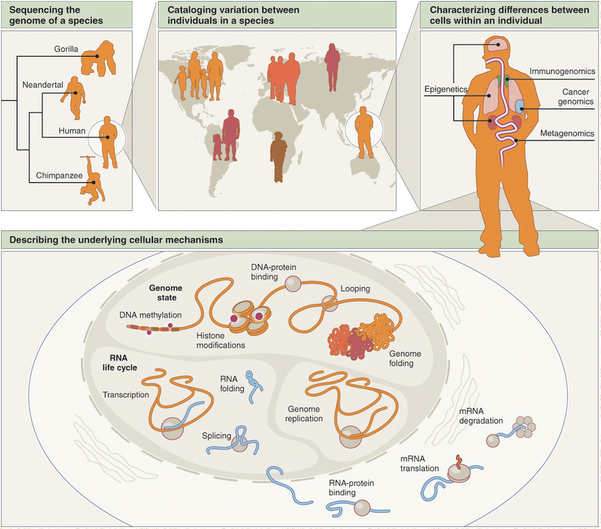
\includegraphics[scale=0.5]{shendure}}
\caption{Les NGS permettent de travailler à différentes échelles\citep{shendure2012expanding}}
\end{figure}

En effet, les méthodes traditionnelles en génétiques des populations ne mettaient en lumière que les effets de la \textbf{dérive génétique} (fixation d'un allèle (une des versions différentes d'un même gène) dans la population), les \textbf{mutations} et les \textbf{migrations}. Mais c'est l'avènement des NGS qui a permis de prendre en compte les effets de la sélection, mais aussi à \citep{bazin2006population} et à \citep{kashi2006simple} de remettre en question ces anciennes pratiques. 

De nouvelles formes de NGS apparaissent rapidement, baissant toujours plus les coûts et les temps de séquençage. Cette évolution est encore plus rapide que la conjecture (loi) de Moore (voir figure \ref{moore}), en effet, en dix ans, le prix d'un séquençage a été divisé par 100 000.

\begin{figure}[!ht]
\centering{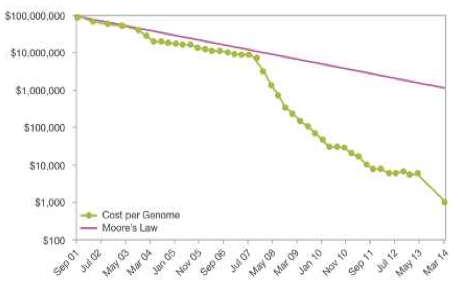
\includegraphics[scale=0.5]{evolution}}
\caption{Evolution très rapide des instruments, des débits et des coûts (premier séquençage sur 454 en Janvier 2008)\label{moore}}
\end{figure}

<< moore_scriptBSB_modifié.R [, options] >>=
     gg4
   @

La qualité et la quantité des résultats a donc explosé. Avec la \textbf{technique Sanger} (première technique de séquençage ADN, en 1977 par Frédérick Sanger) 96 ADNs différents pouvaient être analysés en une fois, alors qu'avec les NGS ce sont des millions d'ADNS différents qui peuvent être analysés en une fois. C'est un véritable saut technologique.

Il existe de nombreuses technologies et plateformes dont les principales sont la technique de \textbf{pyroséquençage 454} (Société Roche, avec les appareils GS Junior System, et GS FLX+ System), la technique d'\textbf{Illumina} (Société Solexa avec les appareils HiSeq System, Genome analyser Ilx ou encore MySeq), la technique  \textbf{Applied Biosystems} de Life Technologies avec les appareils SOLID 5500 System ou encore la technique \textbf{Ion Torrent} de la même société (Life Technologies, avec les appareils Personal Genome Machine et Proton). À partir de 2012, une nouvelle génération de séquenceur encore plus performant arrive sur le marché, appelé ``troisième génération de séquenceur'' ou encore ``\textbf{Next-Next Generation Sequencing}''. Les principales techniques sont celles d'\textbf{Helicos} (avec l'appareil Helicos Genetic Analysis System), la technique \textbf{Pacific Biosciences} avec PacBio RS ou encore la technique d'\textbf{Oxford Nanopore Technologies} avec GridION System et MinION. 

Il ne sera présenté ici que la technique de pyroséquençage 454, la technique d'Illumina via la technique RAD-Seq et la technique d'Oxford Nanopore via le MinION.

Toutes ces NGS se basent sur le même principe. Il faut \textbf{fragmenter} l'ADN, créer des \textbf{banques d'ADN} par ligation d'adaptateurs, les \textbf{cloner} (soit par PCR en émulsion sur une bille dans des microréacteurs (décrit plus bas, dans la technique 454) comme pour les techniques 454 ou SOLID, ou alors par ``Bridge'' PCR (Polymerase Chain Reaction) sur un support plan (Flow cell) ce qui permet de créer des colonies d'ADn se nommant polonies, comme dans la technique Illumina), puis ces clones sont \textbf{séquencés} par une des techniques vu précedemment. Par réaction chimique, de la luminescence est émise (décrit plus bas, dans la technique 454) ce qui permet de convertir les séquences en fichier informatique.

%\subsection{Le pyroséquençage, exemple de la technique 454}
~~\\

En 2005, Jonathan M. Rothberg a élaboré la technologie de \textbf{pyroséquençage 454} Life Sciences (depuis racheté par Roche) et a prouvé la robustesse de ce séquençage en séquençant le génome de \textit{Mycoplasma génitalium} \citep{Margulies2005aa} et qui ne nécessite pas de clonage (donc gain de temps et d’argent), et permet une lecture directe de la séquence obtenue après le séquençage.\citep{sengenes2012developpement}.

La particularité de cette technologie est qu'elle repose sur trois phases, dont une phase centrale de PCR en émulsion pour l'amplification des fragments à séquencer. \citep{Margulies2005aa} \citep{sengenes2012developpement}

La première phase correspond à la \textbf{préparation de la banque:} L’ADN que l'on souhaite séquencer est dans un premier temps fragmenté par nébulisation \citep{loman2012performance} (pour les petits ADN de \unit{0.5-5}{\micro\metre}\citep{Prodromou2007aa}, et utilisé avec de l'azote comprimé)\citep{syed2009next} , par audition hydrodynamique \citep{poptsova2014non} (pour les ADN de taille moyenne \unit{5-10}{\micro\metre})\citep{Prodromou2007aa} qui est obtenu à l'aide de pressions aquatiques exercées sur les molécules d'ADN \citep{poptsova2014non} ou par ``sonication'' \citep{Knierim2011aa} (pour les gros ADN de \unit{10-100}{\micro\metre})\citep{Prodromou2007aa} où les échantillons sont soumis à des ondes ultrasonores, dont les vibrations produisent des cavitations gazeuses dans le liquide qui cisaillement les molécules d'ADN par vibration de résonance \citep{Knierim2011aa}. afin d'obtenir des fragments d'environ 300pb. Les extrémités cohésives créent lors de la coupure vont être réparées afin d’obtenir des extrémités franches permettant l’ajout des adaptateurs.\citep{Prodromou2007aa} \citep{sengenes2012developpement}

Par le biais d'une ADN ligase \citep{sengenes2012developpement}, on ajoute ensuite des adaptateurs qui contiennent notamment une séquence MID (Multipled IDentifier) qui permettra d'identifier chaque échantillon lors du séquençage. \citep{Margulies2005aa}

La seconde phase est l'\textbf{amplification clonale par PCR (Polymerase Chain Reaction) en émulsion (emPCR):}

La PCR à lieu dans une microgoutte avec une microbille d'agarose en phase aqueuse, baignant dans de l'huile avec plusieurs autres millions de billes. Chaque bille comprend donc plusieurs copies d'un même brin d'ADN. Chacune des billes est disposée dans un des 1,6 millions de puits d'un support nommé PTP (PicoTiterPlate) \citep{sengenes2012developpement}

La dernière phase correspond à la \textbf{réaction de séquençage en elle même qui est le pyroséquençage:} ces réactions se produisent dans chaque puits avec les nucléotides qui traversent l'un après l'autre la PTP (voir figure \ref{1}). Quand la polymérase incorpore un nucléotide, un pyrophosphate (PPi) est alors libéré, et par le biais de cascades enzymatiques, une adénosine triphosphate (ATP) est crée qui va ensuite convertir la luciférine en oxyluciférine via une luciférase. C'est cette dernière réaction qui produit de la lumière, et plus de nucléotides seront incorporés, plus la réponse lumineuse sera importante. Ces signaux lumineux sont captés par la machine qui les convertis en information numérique. \citep{sengenes2012developpement}

Cette technique présente malgrè tout des limitations:

\begin{itemize}
\item \textbf{Pour l'extraction des données:} un fichier SFF (Standard Flowgram File) est créé en sortie standard du 454 (Fichier binaire qui est humainement illisible\citep{Peyretaillade2010}), pour le lire il faut un exécutable fourni par la société Roche (sffinfo, uniquement pour ordinateurs avec noyeau Unix (Linux, iOs...))
\item \textbf{Les erreurs de séquençage peuvent être nombreuses:} 

\begin{enumerate}
	\item Il existe des {\itshape insertions ou des délétions} qui rendent difficile à déterminer le nombre de nucléotides entrant dans la composition d'un homopolymère (suite d'un même nucléotide), possible perte de la relation de linéarité entre l'intensité lumineuse émise et le nombre de nucléotides incorporé \citep{Peyretaillade2010}. Il peut aussi y avoir détection d'un signal provenant d'un puits adajacent \citep{Peyretaillade2010}. Selon \citep{balzer2011systematic}, le \textbf{phénomène de CAFIE} (CArry Forward/incomplete Extension) est une erreur de séquençage (qui rend les séquences incomplètes) relativement commune.
	\item Des {\itshape bases ambigües} peuvent apparaitre dans la séquence sous forme de code particulier (par exemple un "N" correspond à une base inconnue, ou encore un Y correspond à une hésitation entre les bases C et T...(Communication personnelle; Amélia Viricel-Pante)) 
	\item Des {\itshape erreurs de prédiction} sont aussi possible comme un signal surestimé suivi d'un signal sous-estimé ou vice versa. \citep{gilles2011accuracy}
	\end{enumerate}

\item \textbf{Par des réplicas artificiels:} ils correspond 4 à 44 pourcents des erreurs selon \citep{niu2010artificial} et 11 à 35 pourcents selon \citep{gomez2009systematic}). Il y a plusieurs billes dans une même goutte d’émulsion dont une seule porte un fragment d’ADN. La caméra détecte une émission de lumière dans un ou plusieurs puits vides provenant d’un puits adjacent où s’effectue la réaction de pyroséquençage \citep{Peyretaillade2010}.
\item Et enfin il existe des \textbf{séquences chimériques (amplicons)}, qui sont des séquences qui se sont hybridées\citep{haas2011chimeric}.
\end{itemize}

En 2005, Rothberg annonça que cette technologie permettrait de séquencer le génome de James D. Watson pour seulement 1 millions de dollars \citep{Margulies2005aa} \citep{sengenes2012developpement}.
Ils réussirent en 2007 en respectant le budget annoncé, et en le réalisant en deux mois \citep{wheeler2008complete}. En 2006, c'est avec cette technique que le génome de l'homme de Néanderthal à pu être séquencé \citep{green2006analysis}, \citep{noonan2006sequencing}, même si \citep{Wall2007aa} ont démontré qu'il y avait majoritairement de l'ADN humain moderne contaminant \citep{sengenes2012developpement}.

\begin{figure}[!ht]
\centering{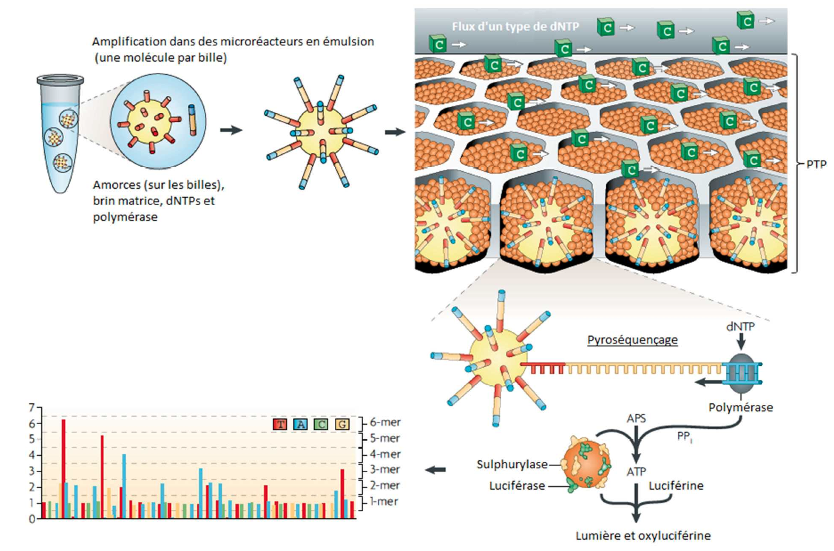
\includegraphics[scale=0.5]{454totale}}
\caption{Aperçu de la technologie 454 \citep{sengenes2012developpement}, PTP: PicoTiter Plate, PPi: pyrophosphate inorganique, APS: adénosine phosphosulphate, ATP: adénosine triphosphate.\label{1}}
\end{figure}

%\subsection{RAD Seq}
~~\\

Les \textbf{marqueurs des sites de restriction} (séquence particulière de nucléotides qui est reconnue par une enzyme de restriction comme un site de coupure dans la molécule d'ADN) associés à l'ADN (\textbf{RAD-Seq}: Restriction site Associated DNA) sont utilisés pour la cartographie génétique, dont la cartographie des QTL (Quantitative Trait Loci), mais aussi dans la génétique des populations, et donc dans la compréhension de l'évolution \citep{davey2010radseq}. 

\begin{figure}[!ht]
\centering{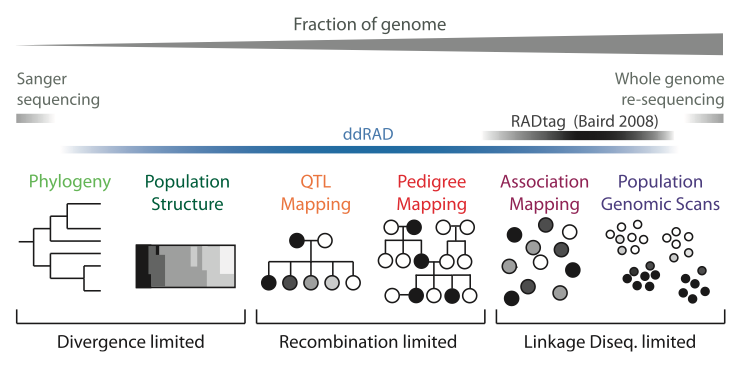
\includegraphics[scale=0.5]{genscan}}
\caption{Résolution des marqueurs de type RAD: Un procédé de génotypage souple peut être utilisé pour optimiser le nombre de marqueurs génétiques pour une approche expérimentale spécifique dans un système biologique donné\citep{peterson2012double}}
\end{figure}

La \textbf{technique RAD-Seq} est un séquençage de type NGS qui lie les séquences aux sites de restriction \citep{Baird2008aa}, puis fragmente le génome par digestion enzymatique, réalise des ligation d'amorces et un code barre (pour distinguer les différents échantillons \citep{davey2013special}). Il faut isoler les balises RAD (\textbf{RAD-tags}), puis les séquences ADN flanquent immédiatement dans chaque site de restriction dans tout le génome. Il y a donc deux fois plus de RAD-tags que de sites de restriction\citep{davey2013special}. Une fois les balises RAD isolées, on identifie et recherche les SNP (Single Nucleotide Polymorphism) pour voir le polymorphisme \citep{hohenlohe2010population}. Il est utilisé sur des séquenceurs de type Illumina, SOLID ou encore Ion Torrent PGM \citep{hohenlohe2010population}. 

\begin{figure}[!ht]
\centering{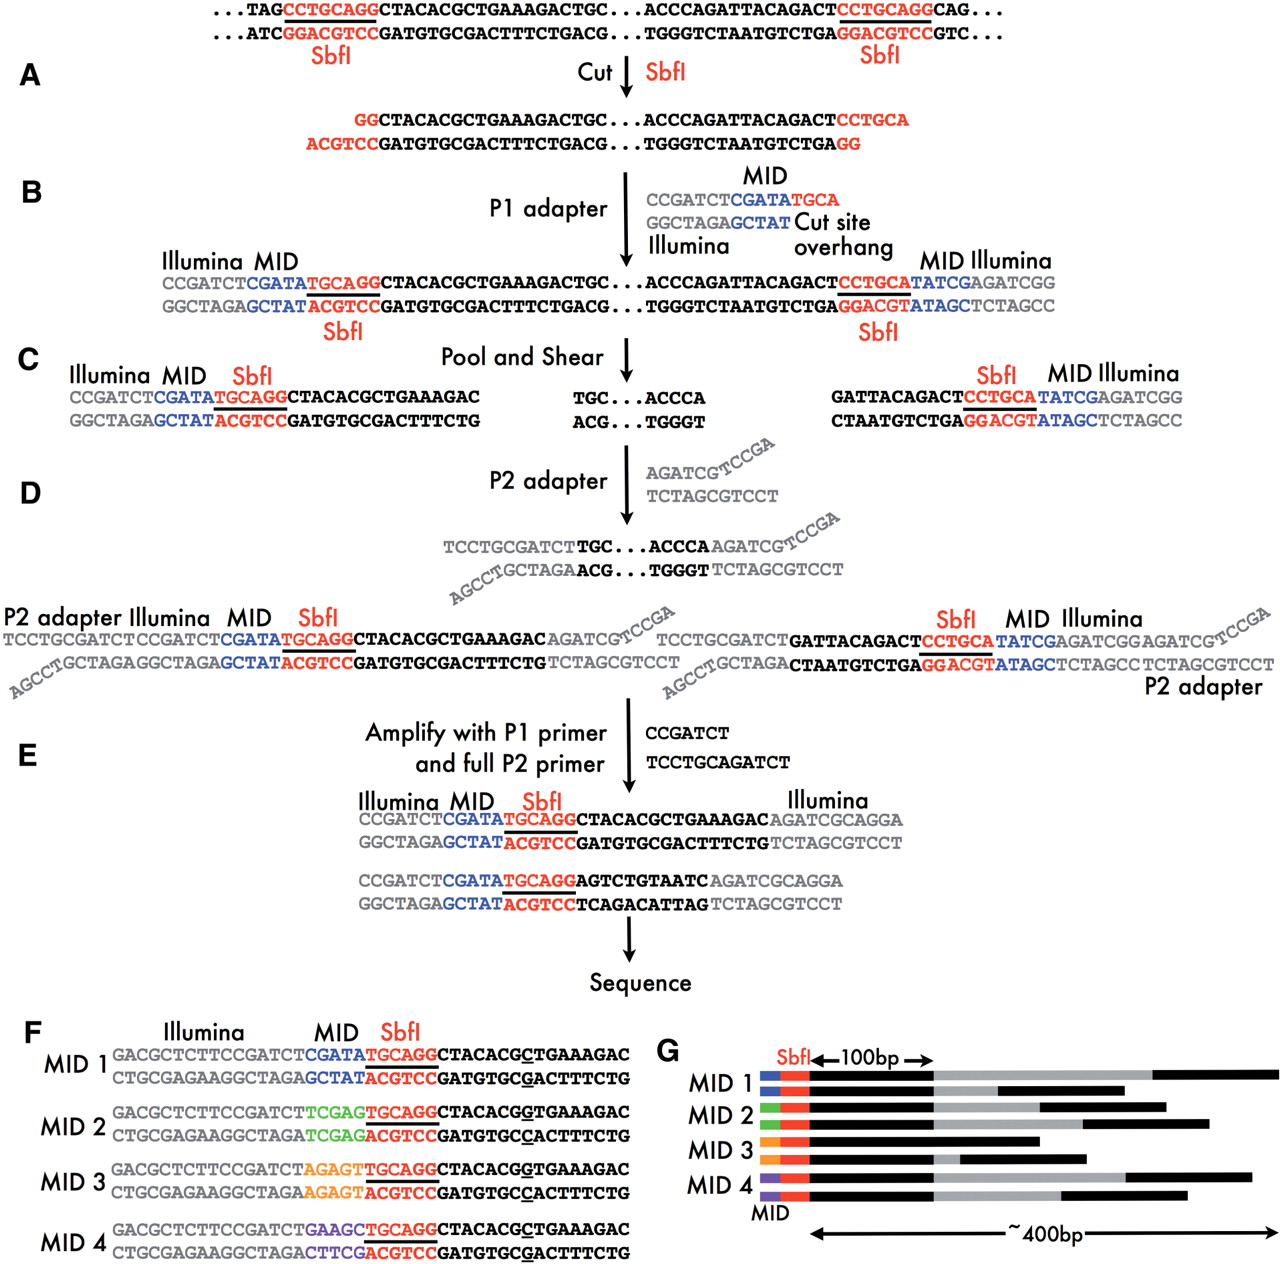
\includegraphics[scale=0.25]{radseq}}
\caption{étapes pour obtenir des séquences d'ADN via la technique Rad seq}
\end{figure}

C'est une technique très utilisée pour la \textbf{biologie évolutive}:

\begin{itemize}
\item \citep{hohenlohe2010population} ont utilisé la \textbf{technique Illumina-sequenced RAD tags} pour identifier plus de 45 000 SNP chez 100 épinoches (\textit{Gasterosteus aculeatus}) provenant de la mer ou de rivières. Cette étude est une première en terme \textbf{scannage génomique} de haute densité basé sur des SNP permettant de calculer la diversité génétique et la différenciation de ces populations d'épinoches dans la nature. Ceci a permit de d'identifier les régions génomiques, d'élucider la part évolutive et démographique de ces populations naturelles et donc de trouver \textbf{des gènes candidats de signification évolutive}. 

\item De la \textbf{cartographie à l'aide de marqueurs} a était réalisé sur des Lepisosteus (\textit{Lepisosteus oculatus})\citep{Amores2011aa}, ce qui a permit de découvrir que c'est une lignée de poissons qui a divergée avant la duplication du génome des téléostéens (ce qui correspond à un "Outgroup"). De plus, cette technique a mis en lumière que leur génome est plus proche de celui des hommes que celui des autres téléostéens (voir figure \ref{2}).

\begin{figure}[!ht]
\centering{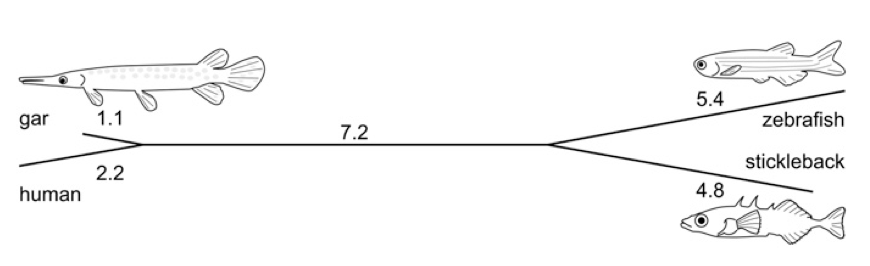
\includegraphics[scale=0.5]{teleo}}
\caption{Comparaison synthetique de deux téléostéens (zebrafish and stickleback) par rapport au lepisosteus et à l'homme. La longueur des branches est proportionnelle à l'estimation du nombre de divergence en terme de chromosome entre les espèces \citep{Amores2011aa}\label{2}.}
\end{figure}


\item Les \textbf{scans génomiques} sur des milliers de SNP peuvent permettre de découvrir un patron de divergence et/ou un flux de gènes entre des espèces écologiquement divergente, comme pour \textit{Populus tremula} avec \textit{Populus trichocarpa} \citep{Stolting2013aa}. Stölting et ses collègues ont scanné le génome de ces deux arbres hybrides différents d'un point de vue écologique. Ils ont utilisé plus de 38 000 SNP en utilisant la méthode de RAD-seq et ils ont découvert une grande divergence génétique (e.g. la proportion de SNP fixé) entre les espèces sur 11 des 19 chromosomes. Ceci correspondrait plus à un flux de gènes régulier qu'a du polymorphisme ancestral partagé. Ces résultats permettent donc d'expliquer l'origine de ces "génomes mosaïques" \citep{Stolting2013aa} vu dans ces taxa avec des génomes dits "poreux" \citep{Stolting2013aa} et suggèrent une introgression ou une conservation extensive naissante parmis les espèces des chromosomes sexuels chez ces végétaux. 

\item Le RAD-seq permet aussi de réaliser de la \textbf{phylogéographie}. En effet, un nombre très large de SNP à travers le génome a le pouvoir d'affiner nos connaissances sur l'histoire démographique d'une population et d'identifier les régions du génome où la sélection naturelle a agit. \citet{Reitzel2013aa} ont utilisé cette technique sur une anémone américaine (\textit{Nematostella vectensis}) en guise de modèle. Des centaines de SNP contenant des "tags" ont été identifiés dans des milliers de RAD loci provenant de 30 individus barcodés de quatre lieux différents sur la côte Est des Etats-Unis d'Amérique. Malgré le manque d'information sur cet espèce (e.g. de génome de référence), un arbre phylogénétique a pu être créé (voir figure \ref{3}) \citep{Reitzel2013aa}.

\begin{figure}[!ht]
\centering{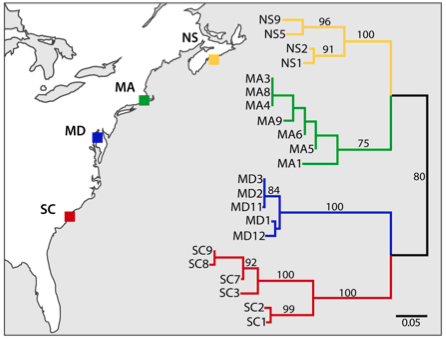
\includegraphics[scale=0.5]{geo}}
\caption{Phylogéographie de \textit{N. vectensis}: Nova Scotia (NS), Massachusetts (MA), Maryland (MD), and South Carolina (SC) \citep{Reitzel2013aa}\label{3}.}
\end{figure}

\item La \textbf{phylogénomique} a vu ses capacités augmenter grâce à la technique RAD-seq. L'analyse des bibliothèques RAD en utilisant des outils bioinformatiques et phylogénétique a permit d'avoir 400 fois plus de sites que l'approche de Sanger et d'avoir par exemple une phylogénie basée sur un alignement de 2 262 825 nucléotides par espèces chez des coléoptères \citep{cruaud2014empirical}. Ainsi les relations entre 18 espèces de carabes qui ont divergé il y a 17 millions d'années ont pu être déterminés avec précision \citep{cruaud2014empirical}, alors que les techniques de Sanger via l'ADN nucléaire et mitochondrial ne donnaient pas les mêmes résultats (voir figure \ref{4}). 

\begin{figure}[!ht]
\centering{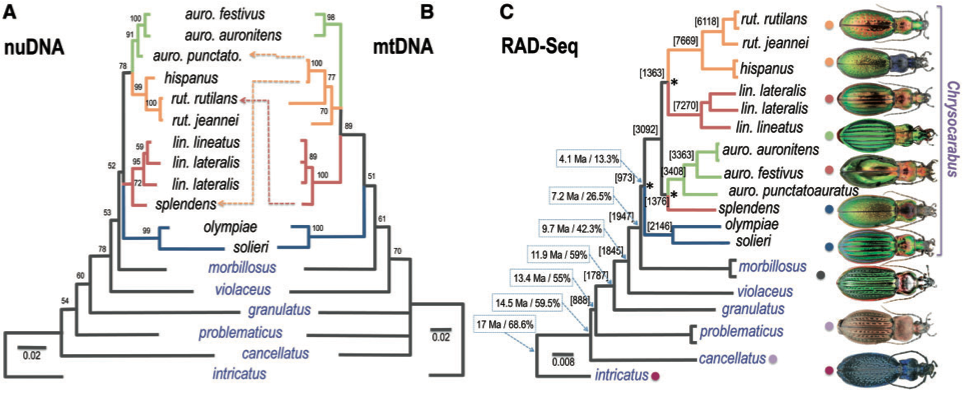
\includegraphics[scale=0.5]{carabe}}
\caption{Phylogénie des carabes obtenues par ADN nucléaire (A), ADN mitochondrial (B) et via la technique de RAD-Seq (C)\citep{cruaud2014empirical} \label{4}.}
\end{figure}

\item C'est aussi une technique très utilisé pour la \textbf{délimitation d'espèces} \citep{herrera2015rad}\citep{Pante2015aa} et la \textbf{structure des populations} \citep{Pante2015aa}. Selon les techniques classiques de génétiques, les \textit{Chrysogorgia} sont des coraux profonds dont les espèces sont délimitées par un seul haplotype mitochondrial \citep{herrera2015rad}\citep{Pante2015aa}. Avec la technique de RAD-Seq le nombre de loci homologues RAD à décru dramatiquement  avec une baisse de la divergence. Plus de 70 pourcents des loci étaient perdus lors de la comparaison de spécimens séparés par deux mutations sur un brin mitochondrial de 700 nucléotides. Ainsi, six espèces sur neuf ont été confirmées, et il se peut que des individus caractérisé par un même haplotype mitochondrial peuvent appartenir à des espèces disctinctes. À l'inverse, trois haplotypes mitochondriaux forment un clade bien supporté dans lequel aucune structure de population n'a été détecté, ce qui suggère une possible variation intraspécifique de l'ADN mitochondrial chez \textit{Chrysogorgia}. Ainsi, les données RAD ont permis à peaufiner les interprétations des marqueurs mitochondriaux classiques utilisés dans les octocoraux pour délimiter les espèces et de découvrir la diversité détectée auparavant \citep{Pante2015aa}.

\end{itemize}

Il existe cependant quelques difficultés liées au génotypage de SNPs RAD-tags \citep{PanteE2014} \citep{mastretta2015restriction}.
En effet, \textbf{en laboratoire}, la qualité des réactifs peut-être hétérogène, les risques de contamination sont possible, des erreurs de pipetage peuvent subvenir, la sensibilité de l’enzyme à la qualité de l’ADN n'est pas toujours la même, ou encore des biais liés aux PCR. \citep{Bonin2004aa}, \citep{Baird2008aa}, \citep{peterson2012double}, \citep{hohenlohe2012extensive}, \citep{PanteE2014}
De plus, il peut y avoir des erreurs \textbf{de séquençage} ou encore un séquençage aléatoire d’allèles et de loci \citep{meacham2011identification}, \citep{nielsen2011genotype}, \citep{hohenlohe2012extensive}, \citep{loman2012performance}, \citep{PanteE2014}.
Il peut aussi y avoir des erreurs \textbf{intrinsèques au génome} comme le polymorphisme sur les sites de restriction ou la méthylation du site de restriction \citep{davey2013special}, \citep{gautier2013effect}, \citep{PanteE2014}.

~~\\

Les \textbf{techniques de Next-Next generation sequencing} qui ont vu le jour en 2012 permettent un séquençage sur une molécule unique et de ce passer de l'amplification clonale \citep{Boyle2014aa}. Cependant, le taux d'erreur de séquençage est 10 fois plus élevé qu'avec le séquençage de type Sanger \citep{Boyle2014aa}. L'appareil \textbf{MinION} (voir figure \ref{minion}) d'\textbf{Oxford Nanopore Technologies} ``deviendra l'approche par défaut du séquençage d'ADN circulaire pour étudier la variété des espèces'' selon \citep{hargreaves2015assessing}. 

Le MinION est un dispositif portable pour les analyses moléculaires grâce à la technologie nanopore. Il est adaptable pour l'analyse de l'ADN, de l'ARN, des protéines ou de petites molécules avec un flux de production simple \citep{nanoport}.

Le principe de la technologie nanopore consiste à faire passer l'ADN le long d'un pore qui est formé par une première protéine qui permet de séparer les deux brins d'ADN (voir figure \ref{nano}) \citep{Boyle2014aa}. Puis le passage de l'ADN simple brin au sein de la seconde protéine provoque un \textbf{courant électrique} caractéristique de chaque base de l'ADN \citep{Boyle2014aa}. Ce courant électrique et ensuite traduit en information numérique \citep{hargreaves2015assessing}. 

Cet appareil à déjà fait ses preuves, notamment pour séquencer rapidement les ARN et ADN de pathogènes comme celui du virus Ebola, donnant des informations scientifiques et sur la santé publique en un temps record \citep{Hoenen2015aa} mais aussi pour réaliser de la taxonomie microbienne de haute résolution et en même temps dans diverses analyses de diversité microbienne via l'étude de l'ADN 16S \citep{benitez2015species}. Ou encore pour la détection en temps réel des gènes de résistance aux antibiotiques, par exemple en cas de pic de Salmonelles dans un hôpital \citep{Quick2015aa}.

\begin{figure}[!ht]
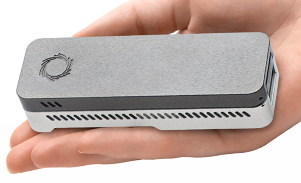
\includegraphics[scale=0.75]{Nanoport} \hfill
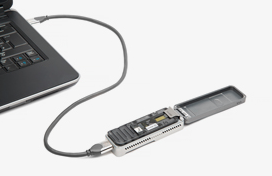
\includegraphics[scale=0.75]{Nanoport2}
\caption{Le MinION \label{minion}}
\end{figure}

\begin{figure}[!ht]
\centering{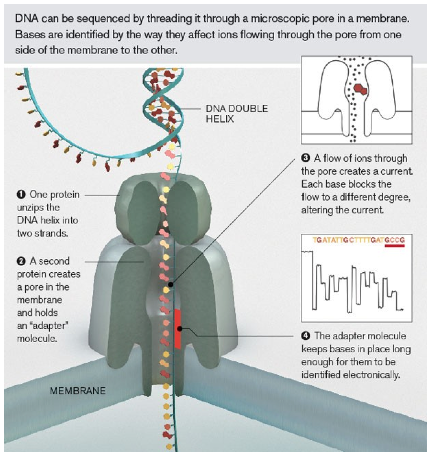
\includegraphics[scale=0.5]{nano}}
\caption{Séquençage de l'ADN via Nanopore\label{nano}}
\end{figure}


%PredRAD: \citep{herrera2014genome} fréquence des sites de coupe extrêmement variable,
%dépend des groupes taxinomiques
%plus le site de coupe est long, moins les sites de coupes sont fréquents sur le génome pas de corrélation claire entre composition en nt du site de coupe et sa prévalence
%prévalence de certains tri-nucléotides meilleur indicateur de fréquence de sites de coupe



%RAD sequencing enables unprecedented phylogenetic resolution and objective species delimitation in recalcitrant divergent taxa \citep{herrera2015rad}

%Conclusions:

%RAD-tag, une représentation réduite du génome
%couplage enzyme de restriction / NGS
%large panel d’utilisations (cartographie -> phylogénétique)
%déclinaisons (e.g. ddRAD) augmentent l’applicabilité
%‣
%compromis rendement / mise en oeuvre / échelle (échantillonnage, phylogénétique...)

%large panel d’outils / pipelines bioinformatiques 

%outils diffèrent par leur stratégies de détection des loci, polymorphisms, allèles

%détection nécessaire des erreurs liés à ces détections (locus drop-out, allele drop-out, genotyping error...)
%‣
%compromis nb marqueurs / taux d’erreur

%stratégies de mise en oeuvre en laboratoire
%--> choix du nb d’individus, de l’enzyme, de la plateforme de séquençage, du nb de runs...
%--> réplicats techniques: individus / banques / séquençage 

%stratégies de traitement bioinformatique des données
%--> choix de la plateforme de traitement, philosophie des outils disponibles (e.g. Stacks vs. PyRAD)
%--> exploration de l’espace paramétrique (e.g. couverture, divergence) et estimation de l’incertitude liée au génotypage




%\section{Mémo notes}

%Apport des NGS pour inférer la structure de population

%--> Qu'est ce que ça nous apprend de plus ?

%Méthodes traditionnelles en génétiques des populations --> Dérive, mutation et migration. --> "On était bien" BSB\copyright

%NGS ont permis de prendre en compte la sélection et ça à mis 30 ans de recherches en question.

%~Basin (2006) --> Taille de la population décorrélé au nombre de diversité mitochondriale --> Il faudrait faire un balayage sélectif
%~~\\
% RAD SEQ --> Moins de marqueur que 454
%Amélia --> Dauphin commun --> Structure population en Atlantique --> Augmentation du nombre de marqueur --> Augmentation de la puissance statistique
%Car génétique ne montrait qu'une seule population, alors que écotoxicologie et isotopes en montraient plusieurs.
%On va travailler sur marqueur de sélection --> Adaptation locale --> Ce sont les marqueurs Outlayer --> FST --> Avec les FST on revient dans un système circulaire (on a deux populations, on veut les différencier, on a un FST, on regarde si c'est supérieur. Aurait-on le même résultats avec 5 population ? Si on a 1000 marqueurs, il y en a forcement --> Statistiques fréquentistes (c'est à l'opposé des statistiques bayésiennes))
%--> On coupe le jeu de données en deux.
%~~\\
%Do it yourself ABC (Marie Louis, usé à la fin de thèse)
%--> Histoire évolutive
%~~\\
%Eric: 
%\begin{itemize}
%\item Séquenceur nanoport (Oxford)
%\item Micness --> Séquence en NGS les microsatelites, Marie Suez et al. 2015
%\end{itemize}

% Séquenceur à plaques --> N'est pas un NGS

% Génome scan 
% Familles de méthodes (pyroseq, rad seq, ce qui est produit par genome scan)
% (faire attention à) différenciation méthode analystique et génétique (quelle couverture du génome on a)
% Voir review NGS, voir en therme d'inférence de structure de pop

%\section{MicNeSs}

%Suez, M., Behdenna, A., Brouillet, S., Graça, P., Higuet, D. and Achaz, G. (2015), MicNeSs: genotyping microsatellite loci from a collection of (NGS) reads. Molecular Ecology Resources. doi: 10.1111/1755-0998.12467
%~~\\
%Les microsatellites sont largement utilisés dans la génétique des populations pour découvrir événements évolutifs récents. Ils sont généralement génotypés en utilisant un séquenceur à capillaire, dont la capacité est généralement limitée à 9, au plus 12 loci pour chaque terme, et dont l'analyse est une tâche fastidieuse qui est effectué à la main. Avec la montée de séquençage de nouvelle génération (NGS), un plus grand nombre de lieux et de personnes sont disponibles à partir de séquençage: par exemple, sur un seul passage d'un GS junior, 28 loci de 96 personnes sont séquencées avec une couverture 30X. Suez et al 2015 ont développé un algorithme pour génotyper automatiquement et efficacement les microsatellites à partir d'un recueil de lectures triés par individu (par exemple amplifications par PCR spécifiques d'un locus ou d'une collection de lit qui englobent un locus d'intérêt). Comme le séquençage et l'amplification par PCR introduisent des insertions ou délétions artefactuelles, l'ensemble de lit à partir d'un seul allèle microsatellite montre plusieurs variantes de longueur. Les déduits de l'algorithme, sans alignement, la vraie inconnue allèle (s) de chaque individu à partir des distributions observées de microsatellites longueur de tous les individus. MicNeSs, une implémentation de Python de l'algorithme, peut être utilisé pour le génotype toute locus microsatellite de tout organisme et a été testé sur 454 données de pyroséquençage de plusieurs loci de mouches des fruits (espèce de modèle) et cerfs rouges (espèce nonmodel). Sans aucune parallélisation, il génotype automatiquement 22 loci de 441 personnes en 11 heures sur un ordinateur standard. La comparaison des inférences MicNeSs la méthode standard montre un excellent accord, avec quelques différences illustrant les avantages et les inconvénients des deux méthodes.


%\section{A creuser}

%Do it yourself: Thèse Marie Louis Chapitre 6, page 162:

%We investigated the demographic history best describing the genetic dataset of the combined microsatellite and mtDNA markers using a coalescent-based Approximate Bayesian Computation (ABC) approach (Beaumont et al. 2002; Bertorelle et al. 2010; Csilléry et al. 2010, the general principle of this analysis is presented in Chapter 2.2c).

%~~\\

%RAD Seq Amélia:

%Amélia Viricel, Eric Pante, Willy Dabin, Benoit Simon-Bouhet. Applicability of RAD-tag geno- typing for inter-familial comparisons: empirical data from two cetaceans. Molecular Ecology Resources, Blackwell, 2014, 14 (3), pp.597-605. <10.1111/1755-0998.12206>. <hal-00908459>

%Viricel, A., & Rosel, P. E. (2014). Hierarchical population structure and habitat differences in a highly mobile marine species: the Atlantic spotted dolphin. Molecular ecology, 23(20), 5018-5035.


\bibliographystyle{mybstfile}
\bibliography{Bibliographie}

\newpage

\section*{Annexe: Historique des technologies}

\begin{itemize}
\item 1953: Découverte de la molécule d'ADN par Watson et Crick
\item 1973: Première séquence de 24 paires de bases publiée (Walter Gilbert and Allan Maxam 1973. The nucleotide sequence of the lac operator)
\item 1975: Southern Blot
\item 1977: Séquençage Sanger & Gilbert
\item 1982: Genbank started
\item 1983: Developpement des PCR (Polymerase Chain Reaction)
\item 1987: Premier sequenceur automatique: Applied Biosystems Prism 373
\item 1990: Séquençage par mesure de la fluorescence
\item 1995: Puces à ADN (microarray)
\item 1996: Sequenceur à capillaires: ABI 310
\item 1998: Genome de \textit{Caenorhabditis elegans} séquencé
\item 2000: Evolution des puces à ADN
\item 2003: Séquençage du génome humain. ~3 milliards de dollars, 13 ans 
\item 2005: 1st 454 Life Sciences Next Generation Sequencing system : GS 20 System
\item 2006 : 1st Solexa Next Generation Sequencer : Genome Analyzer
\item 2007 : 1st Applied Biosystems Next Generation Sequencer : SOLiD
\item 2007: Séquençage d'un individu (JC Venter) Méthode Sanger (Levy et al. Plos Bio 2007)
\item 2008: Séquençage d'un individu (J.D Watson) Méthode haut débit (454 Roche) \citep{wheeler2008complete}, 1 million de dollar, 2 mois
\item 2009 : 1st Helicos single molecule sequencer : Helicos Genetic Analyser System 2011 : 1st Ion Torrent Next Generation Sequencer : PGM
\item 2011 : 1st Pacific Biosciences single molecule sequencer : PacBio RS Systems
\item 2012 : Oxford Nanopore Technologies demonstrates ultra long single molecule reads
\item 2012: "Next-next generation Sequencing"
\end{itemize}


\end{document}


